\documentclass[11pt]{article}
\usepackage[T1]{fontenc}
\usepackage[utf8]{inputenc}
\usepackage{lmodern}
\usepackage{amsmath,amssymb,amsthm,mathtools}
\usepackage[a4paper,margin=28mm]{geometry}
\usepackage{microtype,booktabs,array,enumitem}
\usepackage[numbers,sort&compress]{natbib}
\usepackage{tikz}
\usetikzlibrary{positioning,fit,backgrounds}
\usepackage[colorlinks=true,linkcolor=blue!45!black,citecolor=blue!45!black,urlcolor=blue!45!black]{hyperref}
\hypersetup{pdfauthor={OpenAI},pdftitle={Midpoint convexity from two recursive potentials}}
\setlength{\emergencystretch}{2em}
\newcommand{\R}{\mathbb R}
\newcommand{\N}{\mathbb N}
\newcommand{\E}{\mathbb E}
\newcommand{\PP}{\mathbb P}
\newcommand{\norm}[1]{\left\lVert#1\right\rVert}
\newcommand{\abs}[1]{\left\lvert#1\right\rvert}
\newcommand{\whdelta}{\widehat\delta}
\newcommand{\bardelta}{\overline\delta}
\DeclareMathOperator{\cof}{cof}
\DeclareMathOperator{\supp}{supp}
\newtheorem{theorem}{Theorem}[section]
\newtheorem{lemma}[theorem]{Lemma}
\newtheorem{proposition}[theorem]{Proposition}
\newtheorem{corollary}[theorem]{Corollary}
\theoremstyle{definition}
\newtheorem{definition}[theorem]{Definition}
\theoremstyle{remark}
\newtheorem{remark}[theorem]{Remark}
\numberwithin{equation}{section}
\title{Midpoint convexity from two recursive potentials}
\author{OpenAI}
\date{September 27, 2026}
\begin{document}
\maketitle
\begin{abstract}
We study tree norms computed by two least nonnegative fields whose difference
is the vector. For Euclidean child aggregation, two root-sum spaces have an
averaged asymptotic midpoint modulus of at least $t^3/128$ for $0<t<1$,
including a reflexive joining-root space. A reflexive construction with a
fixed zero root also satisfies a homogeneous cubic estimate. These spaces
admit no equivalent asymptotically uniformly convex norm. We also obtain
sixth-power and cubic estimates when the aggregation exponent depends on
the height of a finite component.
\end{abstract}
\section{Introduction}\label{rec:intro}

A recursively defined norm can be easy to evaluate at one node while
its estimates deteriorate as the tree grows. We study a recursion in
which two nonnegative fields encode a vector as their difference.
Each field at a node dominates the norm of its values at the children,
and the recursion chooses the least feasible pair. For Euclidean child
aggregation, one of the two inequalities is consequently tight at
every node. We show that this local equality controls midpoint
perturbations uniformly in the height and branching of the tree.

For an infinite-dimensional real Banach space $X$ with norm $N$, let
$\operatorname{cof}(X)$ denote its closed finite-codimensional linear
subspaces. The averaged asymptotic midpoint modulus is
\begin{equation}\label{intro:modulus}
 \widehat\delta_N(t)=\inf_{N(x)=1}\sup_{F\in\operatorname{cof}(X)}
 \inf_{\substack{y\in F\\N(y)\ge1}}
 \left(\frac{N(x+ty)+N(x-ty)}2-1\right),\qquad t>0.
\end{equation}
It measures the mean increase in the endpoint norms when a perturbation
avoids a suitable finite-dimensional part of the space. The usual
asymptotic midpoint modulus $m_N(t)$ uses the maximum of the two
endpoint norms, with unit directions, in the same infimum and supremum.
The norm is \emph{asymptotically midpoint uniformly convex}, abbreviated
AMUC, if $m_N(t)>0$ for every $t>0$. This condition was introduced by
Dilworth, Kutzarova, Randrianarivony, Revalski, and Zhivkov
\cite[Definition~2.2]{DKRRZ2016}.
The one-sided modulus is
\begin{equation}\label{intro:auc}
 \overline\delta_N(t)=\inf_{N(x)=1}\sup_{F\in\operatorname{cof}(X)}
 \inf_{\substack{y\in F\\N(y)=1}}\bigl(N(x+ty)-1\bigr).
\end{equation}
A norm is asymptotically uniformly convex, abbreviated AUC, if this
last quantity is positive for every $t>0$.

The averaged and maximum midpoint moduli have the same positivity
property, with
\begin{equation}\label{intro:comparisons}
 \tfrac12m_N(t)\le\widehat\delta_N(t)\le m_N(t).
\end{equation}
Indeed, average is at most maximum. For the converse, at a fixed unit
center intersect a witnessing subspace with the kernel of a norming
functional. Both endpoint norms are then at least one, and their
average excess is at least half the maximum excess. Taking the
infima and suprema proves \eqref{intro:comparisons}.
For a fixed direction, the mean of the two endpoint norms is an even
convex function of the radius. It is therefore nondecreasing on the
positive half-line. Thus the inner infimum in \eqref{intro:modulus}
can equally use $N(y)=1$, and $\widehat\delta_N$ is nondecreasing.
In particular, positivity for $0<t<1$ implies positivity at every radius.

The distinction from AUC renormability is already established.
Dilworth and coauthors separated the two norm properties on $\ell_2$
and posed the corresponding renorming question
\cite[Theorem~2.4 and Section~5]{DKRRZ2016}.
Baudier answered the general question negatively by using the
Kadets--Werner modification of the Bourgain--Rosenthal construction
\cite[Theorem~1 and Corollary~1]{Baudier2026}; the underlying construction
is due to Kadets and Werner \cite[Theorem~2.5]{KW2004}.
That example is nonreflexive \cite[Corollary~2.6]{KW2004}.
Our focus is the quantitative geometry of norms given by an explicit
tree recursion. The joining-root versions are reflexive and still
admit no equivalent AUC norm.

Tree norms have a substantial history in Banach-space theory.
James's construction uses sums over disjoint segments of a binary
tree \cite[p.~739]{James1974}; Girardi proved AUC for its canonical
predual and full dual \cite[Theorems~3 and~5]{Girardi2001}.
A closer comparison is the positive tree cone recalled by Banakh,
following Ghoussoub, Maurey, and Schachermayer
\cite[Section~2.I, pp.~28--29]{Banakh2000}: a nonnegative field at a
node dominates the Euclidean norm of its children. That construction
uses interpolation after taking a symmetric convex hull. Here the
vector is the difference of two least such fields, and the norm is an
explicit cost at the root. The defining norm and its completion are
proved directly below.

\paragraph{Results and proof structure.}
Section~\ref{rec:norms} defines three Euclidean constructions, proves
their completion and finite-coordinate projection properties, and
states Theorem~\ref{rec:main}. The first norm takes the sum of the
root fields on the infinite tree. The second joins finite-height components at
a zero coordinate and takes the common root field; it satisfies a
homogeneous cubic inequality. The third keeps a free coordinate at
that joining root and takes the sum. Both root-sum norms have averaged
modulus at least $t^3/128$ for $0<t<1$; the joined space is reflexive.
Distinguishing the root
normalizations is essential to the constants.

The shortest quantitative argument is in Section~\ref{rec:energy}.
Averaging the fields at $x+z$ and $x-z$ increases both fields of $x$
by the same nonnegative amount $d_s$ at node $s$. Writing $P_s,Q_s$ for
the fields of $x$, the expression
\[
 [d_s(2P_s+d_s)(2Q_s+d_s)]^{2/3}
\]
dominates the sum of its values at the children, by H\"older's
inequality and the tight child inequality. Iterating to the first
nodes outside a finite initial set containing the support of the center
controls the complete tail
by the defect at the root. No factor is multiplied once per level.
Section~\ref{rec:obstruction} supplies the bounded-path argument that
excludes AUC renormings.

Section~\ref{rec:martingale} gives a second way to propagate the same
root-sum defect. A finite stopping rule separates paths according to
the smaller field, a product of field ratios, and the local increase.
An absorbing martingale controls the small-product event. The proof
is uniform over the finite head and retains the order of its parameter
limits. Section~\ref{log:section} gives a different argument on the
joined tree: a logarithmic transform of two bounded supermartingales
bounds a product of ratios and proves a gap for infinite separated
midpoint families.
The stopping proof uses a predictable martingale transform, a classical
tool studied by Burkholder \cite{Burkholder1966}. In the logarithmic proof,
the selected supermartingale increments split into predictable drift and
centered martingale differences. The exact
finite square identities and stopping estimates used here are proved
in place. These arguments explain distinct mechanisms for uniformity, even
though the cubic bound already proves positive midpoint modulus.

Finally, Section~\ref{var:section} replaces Euclidean aggregation
inside a height-$h$ component by $\ell_{1+1/h}$ aggregation. This
exponent is constant inside each component. Two propagation arguments
control different energies: normalized iteration yields a sixth-power
estimate, while accumulated layer energy yields a cubic estimate with
coefficient $(6e)^{-3}$. Their complete proofs include the outer
$\ell_2$ sum and the precise finite-head and weakly null tail statements.
The cubic estimate also gives a cubic lower bound for the averaged
midpoint modulus of this variable-exponent space.

\section{The fields, the roots, and the completed spaces}\label{rec:norms}

Our first objective is to define the norms to which the estimates apply.
All scalars are real. A rooted tree has a distinguished root, and every
node has finitely many predecessors. Its set of children is denoted by
$\operatorname{ch}(s)$. We allow countably many children.
For a finitely supported vector $v=(v_s)$, set the fields to zero below
its support and compute upwards:
\begin{align}
 A_s(v)&=\Bigl(\sum_{c\in\operatorname{ch}(s)}P_c(v)^2\Bigr)^{1/2},&
 B_s(v)&=\Bigl(\sum_{c\in\operatorname{ch}(s)}Q_c(v)^2\Bigr)^{1/2},\notag\\
 P_s(v)&=\max\{A_s(v),v_s+B_s(v)\},&
 Q_s(v)&=\max\{B_s(v),-v_s+A_s(v)\}.
 \label{rec:definition}
\end{align}
Only the finite predecessor closure of the support has nonzero fields.
Empty sums are zero. Thus this instruction is independent of the depth
at which the upward computation starts. At every node,
\begin{equation}\label{rec:field-properties}
 P_s(v)-Q_s(v)=v_s,\qquad P_s(v)\ge A_s(v),\qquad Q_s(v)\ge B_s(v),
\end{equation}
and at least one of the last two inequalities is an equality.
Indeed, subtracting $v_s$ from the formula for $P_s$ gives the formula
for $Q_s$. If the maximum for $P_s$ selects its first entry, its inequality
is tight; otherwise the inequality for $Q_s$ is tight.
Induction also shows that this is the coordinatewise least nonnegative
pair with the prescribed difference and child lower bounds.

\subsection{Three Euclidean constructions}

The local rule is the same in the following spaces, but the underlying
trees and the values taken at the root differ.
\begin{enumerate}[label=\textup{(\roman*)}]
\item On $T=\N^{<\omega}$, including the root $o=\varnothing$, put
\[
 N_\Sigma(v)=P_o(v)+Q_o(v),\qquad v\in c_{00}(T),
\]
and let $X_\Sigma$ be the completion.
\item Let $T_n=\bigcup_{j=0}^n\N^j$, $n\ge1$, be disjoint copies with
roots $r_n$. Add a root $\rho$ whose children are the $r_n$, obtaining a
tree $\mathcal J$. For vectors on $\mathcal J\setminus\{\rho\}$ set
$v_\rho=0$. Then $P_\rho(v)=Q_\rho(v)$; define
\[
 N_0(v)=P_\rho(v)=Q_\rho(v),
\]
and let $X_0$ be the completion.
\item\label{rec:joined-sum-definition}
On the same tree $\mathcal J$, now allowing the coordinate $v_\rho$ to
vary, put
\[
 N_J(v)=P_\rho(v)+Q_\rho(v),\qquad v\in c_{00}(\mathcal J),
\]
and let $X_J$ be the completion.
\end{enumerate}
In particular, $N_J(v)=2N_0(v)$ on the subspace where $v_\rho=0$.
Allowing that coordinate to vary produces an additional one-dimensional
part; it does not change the local recursion.

We call a finite root-containing set \emph{initial} if it contains all
predecessors of its nodes, write $\Pi_H$ for coordinate restriction,
and put $F_H=\ker\Pi_H$ in the corresponding completion.
The next theorem gives the principal quantitative conclusions. The definition
of $\widehat\delta$ is \eqref{intro:modulus}.

\begin{theorem}\label{rec:main}\label{rec:joined-root-stability}
For $N=N_\Sigma$ on $X_\Sigma$, or $N=N_J$ on $X_J$, one has
\begin{equation}\label{rec:sum-modulus}
 \widehat\delta_N(t)\ge t^3/128\qquad(0<t<1).
\end{equation}
For $X_0$, a finite initial set $H$, a vector $x$ supported in $H$, and
$z\in F_H\setminus\{0\}$, one has
\begin{equation}\label{rec:equal-estimate}
 \frac{N_0(x+z)+N_0(x-z)}2\ge N_0(x)
 +\frac{N_0(z)^3}{8(2N_0(x)+N_0(z))^2}.
\end{equation}
Each of $X_\Sigma,X_0,X_J$ admits no equivalent AUC norm.
\end{theorem}

The energy proof in Section~\ref{rec:energy} gives the first two
assertions, uniformly in the height and branching of $H$.
Section~\ref{rec:obstruction} proves the last assertion by following
bounded paths whose next increments are weakly null. The two later
probabilistic arguments obtain uniform separation by controlling the
propagation along random paths.

\begin{proposition}\label{rec:completion}
These formulas define infinite-dimensional Banach spaces after completion.
Coordinate evaluations and the fields extend continuously. If $H$ is a
finite set containing the root and all predecessors of its nodes, then
coordinate restriction $\Pi_H$ is a contractive projection. Its kernel
$F_H$ has finite codimension, and finitely supported elements of $F_H$
are dense in $F_H$. Both $X_0$ and $X_J$ are reflexive.
\end{proposition}

\begin{proof}[Proof of Proposition~\ref{rec:completion}]
The fields are positively homogeneous and subadditive. To verify
subadditivity, induct upwards: the child Euclidean norms are monotone
on nonnegative arrays and satisfy the triangle inequality. Each entry
in either maximum in \eqref{rec:definition} is therefore subadditive,
and a maximum of two subadditive functions is subadditive. Negation
interchanges $P_s$ and $Q_s$. This proves symmetry and the triangle
inequality for each proposed norm. Moreover,
\[
 |v_s|\le\max\{P_s(v),Q_s(v)\}\le N(v),
 \qquad N\in\{N_\Sigma,N_0,N_J\},
\]
by following the child inequalities to the corresponding root.
This proves definiteness and coordinate continuity. The coordinate
vectors are linearly independent, so the spaces are infinite dimensional.

The fields of $\Pi_Hv$ vanish outside $H$. Inside $H$ its coordinates
are unchanged, and each maximum is nondecreasing in the child fields;
induction gives $P_s(\Pi_Hv)\le P_s(v)$ and the same for $Q_s$.
Thus $\Pi_H$ is contractive. Ignore the fixed coordinate $\rho$ when
$N=N_0$. It extends to the completion and has finite-dimensional range.
Applying $I-\Pi_H$ to finite approximations proves tail density.
Choose an increasing sequence $(H_k)$ of finite initial sets covering
the tree. If a finite vector $v$ is supported in $H_k$, then
\[
 N(x-\Pi_{H_k}x)
 \le N(x-v)+N(\Pi_{H_k}(v-x))\le2N(x-v).
\]
Density therefore gives $\Pi_{H_k}x\to x$ for every completed vector
$x$. In particular, the coordinates separate points. A completed
vector whose coordinates vanish outside a finite initial set $H$
equals $\Pi_Hx$, so support in $H$ has its usual coordinate meaning.
Subadditivity and sign exchange give
\[
 |P_s(v)-P_s(w)|\le N(v-w),\qquad
 |Q_s(v)-Q_s(w)|\le N(v-w).
\]
The fields therefore extend continuously, and the root norm formulas
persist on the completions.

We prove reflexivity by describing the finite-height components. Set
$M_n(v)=\max\{P_{r_n}(v),Q_{r_n}(v)\}$ on $c_{00}(T_n)$, and let
$E_n$ be its completion under this norm.
Writing $m_s=\max\{P_s,Q_s\}$ gives
\[
 m_s\le |v_s|+\Bigl(\sum_{c\in\operatorname{ch}(s)}m_c^2\Bigr)^{1/2}.
\]
The Euclidean norm of the $m_s$ on one level is at most the Euclidean
norm of the coordinates on that level plus the corresponding norm of
$m_c$ on the next level. Iteration and Cauchy--Schwarz yield
$M_n(v)\le\sqrt{n+1}\,\|v\|_2$.
Conversely the $\ell_2$ norm of either field on any level is at most its
root value. Since $v=P-Q$,
\begin{equation}\label{rec:block-equivalence}
 \frac{\|v\|_2}{2\sqrt{n+1}}\le M_n(v)
 \le\sqrt{n+1}\,\|v\|_2.
\end{equation}
Hence $E_n$ is $\ell_2(T_n)$ with an equivalent norm,
and is reflexive. The recursion extends to its vectors by continuity
or directly by the finitely many levels.

For $v$ with zero joining coordinate, put
$L(v)=(\sum_n M_n(v|_{T_n})^2)^{1/2}$. The two child arrays at $\rho$
give
\begin{equation}\label{rec:joined-equivalence}
 N_0(v)\le L(v)\le\sqrt2\,N_0(v).
\end{equation}
For a free root coordinate $a=v_\rho$, with the remaining coordinates
written as $w$, let
$A=(\sum_nP_{r_n}(w)^2)^{1/2}$ and
$B=(\sum_nQ_{r_n}(w)^2)^{1/2}$.
Then
\begin{equation}\label{rec:free-root-equivalence}
 N_J(v)=\max\{2A-a,2B+a\},\qquad
 \max\{|a|,L(w)\}\le N_J(v)\le |a|+2L(w).
\end{equation}
For the lower bound, $N_J\ge |a|$ and $N_J\ge A+B\ge L(w)$.
These comparisons identify $X_0$ with the $\ell_2$ sum of the $E_n$
under an equivalent norm, and $X_J$ with that sum plus $\R$.
The Hilbert comparisons for individual components need not be uniform
in $n$: we take the outer sum in the norms $M_n$ themselves.

For completeness, an $\ell_2$ sum of Banach spaces is complete:
a Cauchy sequence converges in each component, and its Cauchy bounds
pass to all finite component sums and then to their supremum. Its dual
is the $\ell_2$ sum of the component duals. The upper norm bound is
Cauchy--Schwarz; the lower bound follows by testing a functional on
finitely many almost norming component vectors with scalar coefficients
proportional to their dual norms. Finite component vectors are dense.
Applying this dual identification twice proves reflexivity when each
component is reflexive. Equivalent norms preserve reflexivity.
This proves the assertion for both joined spaces.
\end{proof}

\paragraph{Component root sums.}
The alternative norm $P_{r_n}+Q_{r_n}$ lies between $M_n$ and $2M_n$,
so it gives the same component completion. Its behavior on individual
levels can also be read directly from the recursion. For a finite
vector on $T_n$, put $s_a=P_a+Q_a$. Then
\begin{equation}\label{rec:sum-level-bounds}
 \max\{|v_a|,\|(s_c)_{c\in\operatorname{ch}(a)}\|_2\}
 \le s_a\le |v_a|+2\|(s_c)_{c\in\operatorname{ch}(a)}\|_2.
\end{equation}
Indeed, $s_a\ge A_a+B_a\ge\|(s_c)_c\|_2$ and
$s_a=\max\{2A_a-v_a,2B_a+v_a\}$.
Iteration bounds its root value above by
$\sum_{d=0}^n2^d\|v|_{\text{level }d}\|_2$, while each level norm of
$v$ is at most that root value. These provide direct Hilbert comparisons
for the component root-sum convention.

\section{From root defect to boundary energy}\label{rec:energy}

To prove Theorem~\ref{rec:main}, we will compare the fields of the
center with their averages at the two endpoints. The following lemma
is the required calculation. It bounds the squared increases at a
chosen boundary by a quantity measured only at the root.

\begin{lemma}[Two-field energy]\label{rec:two-field}
Let $J$ be a subset of the leaves of a finite tree with root $o$. Suppose that
$P,Q,P',Q'$ are nonnegative fields, each satisfying
\[
 A_s^2\ge\sum_{c\in\operatorname{ch}(s)}A_c^2
\]
at every internal node, for each $A\in\{P,Q,P',Q'\}$. Suppose also that $P'-P=Q'-Q=d\ge0$, and
that at each internal node at least one of the inequalities for $P,Q$
is an equality. If $P_b=Q_b=0$ for $b\in J$, then
\[
 \sum_{b\in J}d_b^2
 \le\bigl[d_o(2P_o+d_o)(2Q_o+d_o)\bigr]^{2/3}.
\]
\end{lemma}

\begin{proof}
Put $E_s=[d_s(2P_s+d_s)(2Q_s+d_s)]^{2/3}$. We show that
$E_s\ge\sum_c E_c$. Suppose first that $P_s^2=\sum_cP_c^2$, and put
\[
 U_s=(P'_s)^2-P_s^2=d_s(2P_s+d_s),\qquad
 V_s=(Q'_s+Q_s)^2=(2Q_s+d_s)^2.
\]
Use the same definitions at the children. The upper inequality for
$P'$ and the equality for $P$ give $U_s\ge\sum_c U_c$. The triangle
inequality in $\ell_2$ applied to the child fields $Q',Q$ gives
$V_s\ge\sum_c V_c$. Consequently H\"older's inequality yields
\[
 \sum_c E_c=\sum_c U_c^{2/3}V_c^{1/3}
 \le\left(\sum_c U_c\right)^{2/3}
     \left(\sum_c V_c\right)^{1/3}
 \le U_s^{2/3}V_s^{1/3}=E_s.
\]
If the tight field at $s$ is $Q$, interchange $P,Q$ in this calculation.
At a leaf in $J$, $E_b=d_b^2$. Iterating the inequality through the
finite tree and discarding the nonnegative energies of the other leaves
proves the assertion.
\end{proof}

\begin{lemma}\label{rec:root-sum-stability}
Let $N=N_\Sigma$ or $N=N_J$. Suppose that $x$ is a finitely supported
unit vector and that $z\in F_H$, where $H$ is a finite initial set
containing $\supp x$. If
\[
 d=\frac12\left(\frac{N(x+z)+N(x-z)}2-1\right),
\]
then $d\ge0$ and $N(z)^3\le64d(1+d)^2$.
\end{lemma}

\begin{proof}[Proof of Lemma~\ref{rec:root-sum-stability} and the quantitative assertions of Theorem~\ref{rec:main}]
We use the fields from \eqref{rec:definition}. For a finite head vector $x$ and a finite tail $z$
vanishing on an initial set $H$ containing $\operatorname{supp}x$, set
\[
 P_s=P_s(x),\quad Q_s=Q_s(x),\quad
 P'_s=\tfrac12(P_s(x+z)+P_s(x-z)),\quad
 Q'_s=\tfrac12(Q_s(x+z)+Q_s(x-z)).
\]
The coordinate difference identity and convexity give the same
nonnegative defect $d_s=P'_s-P_s=Q'_s-Q_s$. The averaged fields satisfy
the upper inequalities by the $\ell_2$ triangle inequality. At a first
node $b$ outside $H$, the head fields vanish on its whole subtree, so
\[
 d_b=\tfrac12(P_b(z)+Q_b(z)).
\]
Only finitely many such values are nonzero. Apply
Lemma~\ref{rec:two-field} to the finite relevant part of $H$ and its
first-exit boundary, retaining at each boundary node its already-computed
full-subtree field values. Discard only subtrees where all four fields
vanish. This gives the bound on $\sum_b d_b^2$. Figure~\ref{fig:boundary}
shows the finite part through which the inequality is propagated.
\begin{figure}[tb]
\centering
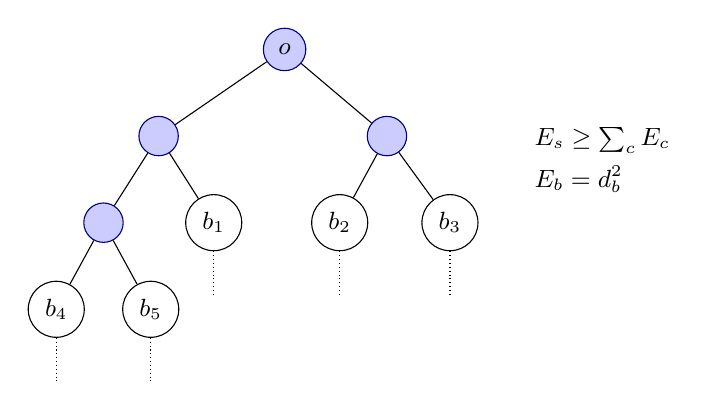
\begin{tikzpicture}[every node/.style={font=\small},
 head/.style={circle,fill=blue!20,draw=blue!50!black,minimum size=5mm},
 boundary/.style={circle,fill=white,draw=black,minimum size=5mm}]
\node[head] (o) at (0,2.2) {$o$};
\node[head] (a) at (-1.6,1.1) {};
\node[head] (b) at (1.3,1.1) {};
\node[head] (c) at (-2.3,0) {};
\node[boundary] (d) at (-0.9,0) {$b_1$};
\node[boundary] (e) at (0.7,0) {$b_2$};
\node[boundary] (f) at (2.1,0) {$b_3$};
\node[boundary] (g) at (-2.9,-1.1) {$b_4$};
\node[boundary] (h) at (-1.7,-1.1) {$b_5$};
\foreach \u/\v in {o/a,o/b,a/c,a/d,b/e,b/f,c/g,c/h}
 \draw (\u)--(\v);
\foreach \v in {d,e,f,g,h} \draw[densely dotted] (\v.south)--++(0,-.55);
\node[align=left,anchor=west] at (3.05,.8) {$E_s\ge\sum_c E_c$\\[4pt]$E_b=d_b^2$};
\end{tikzpicture}

\caption{The shaded nodes form the finite initial set $H$. Each boundary
node $b$ represents its entire descendant subtree: the head vector is zero
there, while the tail fields $P_b(z),Q_b(z)$ have already been computed.
The energy inequality propagates from these boundary values to the root.
The omitted branches contribute zero in a finite-support calculation.}
\label{fig:boundary}
\end{figure}

We next convert this energy into a norm estimate for each of the two
root conventions.
On $H$ the coordinate of $z$ is zero, so $P_s(z)=Q_s(z)$ there. With
$r_s=\max\{P_s(z),Q_s(z)\}$ one has
$r_s^2\le\sum_c r_c^2$ on $H$ and $r_b\le2d_b$ at its boundary.
Thus $r_o\le2(\sum_b d_b^2)^{1/2}$.

\emph{The sum of the root fields.} First use either root-sum space $X_\Sigma$ or $X_J$, and write
$N=N_\Sigma$ or $N=N_J$, respectively. Assume $N(x)=1$ and put
\[
 d=d_o=\frac12\left(\frac{N(x+z)+N(x-z)}2-1\right).
\]
Since $N(z)=2r_o$, the energy lemma gives
\[
 N(z)^3\le64d(2P_o+d)(2Q_o+d)\le64d(1+d)^2.
\]
The last inequality uses $P_o+Q_o=1$. The field continuity and tail
density from Proposition~\ref{rec:completion} extend this cubic inequality to
every $z\in F_H$, with the finite unit center $x$ fixed. This proves
Lemma~\ref{rec:root-sum-stability}. If $N(z)\ge t$
with $0<t<1$, then $d\ge t^3/256$: for $d\le1$ use
$(1+d)^2\le4$, and for $d>1$ the claim is immediate. Since the average
gain is $2d$, it is at least $t^3/128$.

Fix either root-sum space $X\in\{X_\Sigma,X_J\}$ with its norm $N$.
For any unit center $x_0\in X$ and $\varepsilon>0$, choose a
finite unit center $x$ with $N(x-x_0)<\varepsilon$, then choose a finite
initial $H$ containing its support. For all $y\in F_H$ with $N(y)\ge1$,
put $z=ty$ in the preceding estimate. Replacing $x$ by $x_0$ loses at
most $\varepsilon$ in the average, uniformly in $y$. Thus the supremum
over finite-codimensional subspaces at $x_0$ is at least
$t^3/128-\varepsilon$. Letting $\varepsilon\downarrow0$ and taking
the infimum over unit $x_0$ proves \eqref{rec:sum-modulus}.

\emph{The common root field.} Now use $X_0$ and write $N=N_0$,
with $o=\rho$ in the preceding calculation. By definition
$N(v)=P_o(v)=Q_o(v)$. Put
\[
 d=d_o=\frac{N(x+z)+N(x-z)}2-N(x).
\]
Now $N(z)=r_o$, and the same energy lemma yields
\[
 N(z)^3\le8d(2N(x)+d)^2.
\]
The triangle inequality gives $d\le N(z)$. For $z\ne0$ this proves the
homogeneous estimate
\[
 \frac{N(x+z)+N(x-z)}2
 \ge N(x)+\frac{N(z)^3}{8(2N(x)+N(z))^2}.
\]
The tail density from Section~\ref{rec:norms} and continuity extend
this inequality to every nonzero completed tail, proving
\eqref{rec:equal-estimate}.
\end{proof}

The factors eight and sixty-four come from the conversion of boundary
fields into the tail norm: the sum of the root fields introduces a
factor two before cubing. Both estimates therefore depend on the same
local energy inequality, while their root normalizations remain distinct.

\medskip
\noindent\emph{Remark (reciprocal form).}
In the finite-head calculation above, let $\mathcal B$ denote the
first-exit boundary, and retain the fields $P,Q$ and their averaged
increments $d$. For a node $s$ of that finite tree, put
\[
 B_s=\left(\sum_{\substack{b\in\mathcal B\\s\preceq b}}d_b^2\right)^{1/2},
 \qquad w_s^P=2P_s+d_s,\qquad w_s^Q=2Q_s+d_s.
\]
Here $s\preceq b$ means that $s$ lies on the path from the root to $b$,
including $s=b$. Both $w$ fields dominate their child Euclidean norms
and equal $d_b$ at a boundary node, so $w_s^P,w_s^Q\ge B_s$.
Applying Lemma~\ref{rec:two-field} to the descendant subtree rooted at
$s$ gives $B_s^3\le d_s w_s^P w_s^Q$. Thus, whenever $B_s>0$,
\begin{equation}\label{rec:reciprocal-energy}
 d_s\ge\frac{B_s^3}{w_s^P w_s^Q}.
\end{equation}
The undivided inequality is an equality at every boundary node.
This form expresses the same energy estimate through the accumulated
boundary norm $B_s$.

\section{Bounded paths exclude AUC renormings}\label{rec:obstruction}

The midpoint gain controls two opposite perturbations together.
To distinguish it from one-sided asymptotic convexity, we use positive
path vectors that remain bounded as their paths grow. At each stage,
the next coordinate can be chosen from a weakly null sequence of
increments whose norms stay bounded away from zero.

\begin{lemma}[Bounded trees]\label{rec:bounded-tree}
Let $X$ be a Banach space. Suppose that for every $h\ge1$ there are
vectors $u_s^{(h)}$, indexed by $s\in\N^{\le h}$, such that
$0<m\le\|u_s^{(h)}\|\le M<\infty$ uniformly. Suppose also that for
$|s|<h$ the increments
$d_{s,k}^{(h)}=u_{s^\frown k}^{(h)}-u_s^{(h)}$ are weakly null as
$k\to\infty$ and have norms at least $c>0$, uniformly in $h,s,k$.
If $N$ is a norm and $0<\alpha\le\beta<\infty$ satisfy
$\alpha\|\cdot\|\le N\le\beta\|\cdot\|$, then
\[
 \overline\delta_N\left(\frac{\alpha c}{2\beta M}\right)=0.
\]
The conclusion also holds if one infinite tree has these properties.
\end{lemma}

\begin{proof}
Set $t_0=\alpha c/(2\beta M)$ and suppose
$0<\gamma<\overline\delta_N(t_0)$. At a current vector $u_s^{(h)}=u$,
choose a closed finite-codimensional subspace $F$ such that
\[
 N(u+t_0N(u)y)\ge(1+\gamma)N(u)
 \qquad(y\in F,\ N(y)=1).
\]
Convexity extends this inequality to every $w\in F$ with
$N(w)\ge t_0N(u)$. More explicitly, for a unit center $x$ and a unit
direction $y$, convexity at the radii $0,t_0,r$ gives
$N(x+ry)-1\ge(r/t_0)(N(x+t_0y)-1)$ for $r\ge t_0$.

Weak nullity persists under an equivalent norm. In the finite-dimensional
quotient $X/F$ the increments converge to zero in norm, so there are
$w_k\in F$ with $N(w_k-d_{s,k}^{(h)})\to0$.
For large $k$,
$N(w_k)\ge\alpha c/2\ge t_0N(u)$.
Choose $k$ with error less than $\gamma N(u)/2$. The preceding estimate
then gives
\[
 N(u_{s^\frown k}^{(h)})\ge(1+\gamma/2)N(u_s^{(h)}).
\]
Choose $h$ such that $\alpha m(1+\gamma/2)^h>\beta M$ and iterate this
choice for $h$ steps, a contradiction. Restricting an infinite tree to
that height gives the same argument. Finally,
$\overline\delta_N(t_0)\ge0$: intersect a finite-codimensional subspace
with the kernel of a functional norming a given center. Both signs of
every perturbation in that kernel have norm at least that of the center.
\end{proof}

\begin{proof}[Proof of the renorming assertion in Theorem~\ref{rec:main}]
On the infinite tree define
$v_s=\sum_{r\preceq s}e_r$. Along this path the fields of $v_s$ are
$P=1,Q=0$, so $N_\Sigma(v_s)=1$. Its child increments are $e_{sk}$,
and for a finite scalar family $(a_k)$ the recursion gives
\begin{equation}\label{rec:sibling-formula}
 N_\Sigma\Bigl(\sum_k a_ke_{sk}\Bigr)
 =2\max\{\|(a_k^+)\|_2,\|(a_k^-)\|_2\}
 \le2\|(a_k)\|_2.
\end{equation}
Here $a^+=\max\{a,0\}$ and $a^-=\max\{-a,0\}$.
In particular $N_\Sigma(e_{sk})=2$.
The map taking the unit vectors of $\ell_2$ to $e_{sk}$ extends to a
bounded linear map by \eqref{rec:sibling-formula}. Since the unit vectors
of $\ell_2$ are weakly null, so are these increments against every
continuous linear functional on $X_\Sigma$.
Lemma~\ref{rec:bounded-tree} applies with $m=M=1,c=2$.

For a node $s\in T_n$, let $v_s$ be the indicator of the path from
$r_n$ to $s$, with joining coordinate zero. Its component fields are
again $P=1,Q=0$ along the path. At $\rho$ they both equal one. Thus
\[
 N_0(v_s)=N_0(e_s)=1,\qquad N_J(v_s)=N_J(e_s)=2.
\]
At a fixed non-leaf $s$ in a component, the sibling sequence is weakly
null: restricting any functional to that component gives a continuous
functional on a space equivalent to $\ell_2(T_n)$ by
\eqref{rec:block-equivalence}. Alternatively, the sibling computation
in \eqref{rec:sibling-formula} gives a direct bounded map from $\ell_2$;
for $N_0$ its factor two is replaced by one.
The joined trees contain components of every finite height.
Lemma~\ref{rec:bounded-tree} therefore applies to $X_0$ with
$m=M=c=1$, and to $X_J$ with $m=M=c=2$.
In both cases the vanishing one-sided modulus occurs at
$t_0=\alpha/(2\beta)$; for $X_\Sigma$ it occurs at
$t_0=\alpha/\beta$.
\end{proof}

The argument permits the finite-codimensional subspace to change at
every node. Its contradiction uses only a fixed positive gain and
arbitrarily long bounded paths. Reflexivity of the joined constructions
is compatible with this obstruction; it does not imply the existence
of an AUC renorming.

\section{Stopping the propagation of normalized defects}\label{stop:section}\label{rec:martingale}

We return to the root-sum norm $N_\Sigma$ on the infinite tree from
Section~\ref{rec:norms}.  This section gives a second proof that a tail
of fixed size forces a uniform midpoint gain.  Its main object is a
product of ratios along a branch.  We stop the product when either a
normalized base field becomes small, the product becomes small, or an endpoint
defect becomes large.  A finite martingale controls the second kind of
stop; the other two are controlled directly by the fields.

\begin{lemma}[Uniform sequential separation]\label{stop:sequential}
For each $n$, let $x_n,z_n$ be finitely supported real vectors on
$\mathbb N^{<\omega}$, with $N_\Sigma(x_n)=1$.  Let $H_n$ be the
predecessor closure of $\operatorname{supp}x_n$, and suppose that
$(z_n)_s=0$ for every $s\in H_n$.  Then
\[
 \frac{N_\Sigma(x_n+z_n)+N_\Sigma(x_n-z_n)}2\longrightarrow1
 \quad\Longrightarrow\quad N_\Sigma(z_n)\longrightarrow0.
\]
In particular, the assertion is uniform in the height and size of $H_n$.
\end{lemma}

\begin{proof}
We first work with one pair $x,z$, writing $H$ for its head and omitting
$n$.  Write $C_s^1=P_s(x)$ and $C_s^2=Q_s(x)$.  For $s\in H$ define
\begin{equation}\label{stop:normalization}
 w_s=(C_s^1)^2+(C_s^2)^2,\qquad
 \nu_s=\frac{w_s}{w_o},\qquad
 u_s^i=\frac{C_s^i}{\sqrt{w_s}},\qquad
 \ell_s=\min\{u_s^1,u_s^2\}.
\end{equation}
Every subtree rooted in $H$ contains a nonzero coordinate of $x$.
The child inequalities therefore imply $w_s>0$.  At the root,
$1/2\le w_o\le1$, since $P_o(x)+Q_o(x)=1$.
Also $(u_s^1)^2+(u_s^2)^2=1$.  Let $I_s$ be the children of $s$ in
$H$, and $J_s$ the children outside $H$.  Choose an index $i_s\in\{1,2\}$
for which the child inequality of the base vector is tight at $s$.

For $\sigma\in\{-1,1\}$ set
\begin{equation}\label{stop:defects}
 D_s^\sigma=P_s(x+\sigma z)-P_s(x)
             =Q_s(x+\sigma z)-Q_s(x),\qquad
 d_s^\sigma=\frac{D_s^\sigma}{\sqrt{w_s}}\quad(s\in H).
\end{equation}
The two differences agree because $z_s=0$ on $H$.  They are nonnegative:
at exterior children the base fields are zero, and upward induction
uses the monotonicity of the recursion in both child bounds.  Thus
\begin{equation}\label{stop:root-defect}
 N_\Sigma(x+\sigma z)=1+2D_o^\sigma.
\end{equation}
Here and below, $C^1(v)=P(v)$ and $C^2(v)=Q(v)$ when an argument is
specified.  Define the exterior energies by
\begin{equation}\label{stop:exterior}
 E_s^\sigma=\frac1{w_o}\sum_{c\in J_s}C_c^{i_s}(\sigma z)^2,
 \qquad
 \mathcal E=\sum_{s\in H}\sum_\sigma E_s^\sigma
 =\frac1{w_o}\sum_{s\in H}\sum_{c\in J_s}
       \bigl(P_c(z)^2+Q_c(z)^2\bigr).
\end{equation}
Negation interchanges the fields, so the last sum is independent of
our choices of $i_s$.  Only finitely many exterior terms are nonzero.
On $H$ the fields of $z$ agree.  The recursion there gives
\[
 P_s(z)^2=\sum_{c\in I_s}P_c(z)^2+
 \max\left\{\sum_{c\in J_s}P_c(z)^2,
             \sum_{c\in J_s}Q_c(z)^2\right\}.
\]
Telescoping over $H$ proves
\begin{equation}\label{stop:tail-energy}
 N_\Sigma(z)^2\le4w_o\mathcal E.
\end{equation}
We will show that a small root defect forces this exterior energy to
be small, independently of the head.

There is a second useful estimate, for every $a\in H$:
\begin{equation}\label{stop:subtree}
 \sum_{\substack{s\in H\\a\preceq s}}\sum_\sigma E_s^\sigma
 \le\nu_a\sum_\sigma(\ell_a+d_a^\sigma)^2.
\end{equation}
Choose one index $i$ with $u_a^i=\ell_a$, and iterate the child inequality
for the single field $C^i(x+\sigma z)$ from $a$ to all first exterior
nodes below it.  At those nodes the whole base subtree vanishes.
Summing over signs makes the resulting boundary sum independent of
$i$, and division by $w_o$ gives \eqref{stop:subtree}.

\medskip
\noindent\emph{The identity that propagates the defect.}
For a fixed sign abbreviate $d_s=d_s^\sigma$.  Subtracting the tight
base inequality for $C^{i_s}$ from its endpoint inequality yields
\begin{equation}\label{stop:increment}
 \nu_s(2u_s^{i_s}d_s+d_s^2)
 \ge\sum_{c\in I_s}\nu_c(2u_c^{i_s}d_c+d_c^2)+E_s^\sigma.
\end{equation}
Whenever $u_s^{i_s}>0$, put $R_{sc}=u_c^{i_s}/u_s^{i_s}$.
Tightness gives $\sum_{c\in I_s}\nu_cR_{sc}^2=\nu_s$.
Expanding the squares in the following display and using that identity
rewrites \eqref{stop:increment} as
\begin{equation}\label{stop:square}
 2(u_s^{i_s}+d_s)
 \left(\nu_sd_s-\sum_{c\in I_s}\nu_cR_{sc}d_c\right)
 \ge E_s^\sigma+
       \sum_{c\in I_s}\nu_c(d_c-R_{sc}d_s)^2.
\end{equation}
The last sum measures the failure of the defect to propagate by the
ratios $R_{sc}$.  Multiplying those ratios along a branch makes the
left side telescope.

Fix $0<\lambda<1/2$, $0<\zeta<1$, and $h>0$.  Inspect the root with
$Z_o=1$.  At an inspected node $s$, stop when
\begin{equation}\label{stop:rule}
 \ell_s<\lambda,\qquad Z_s<\zeta,
 \qquad\hbox{or}\qquad\max_\sigma d_s^\sigma>h.
\end{equation}
If none holds, call $s$ a continuation node and inspect its children
$c\in I_s$ with $Z_c=Z_sR_{sc}$.  The denominator in $R_{sc}$ is at
least $\lambda$ at such a node.  Let $G$ and $S$ denote the continuation
and stop sets.  Every leaf of $H$ has $\ell_s=0$, so every inspected
branch stops.  The stops are incomparable, and the child inequalities
give
\begin{equation}\label{stop:mass}
 \sum_{T\in S}\nu_T\le1.
\end{equation}
Multiplying \eqref{stop:square} at $s\in G$ by
$Z_s/[2(u_s^{i_s}+d_s^\sigma)]$, which is at least
$\zeta/[2(1+h)]$, and summing gives
\begin{equation}\label{stop:telescope}
 \begin{split}
 \sum_{T\in S}\nu_TZ_Td_T^\sigma
 &+\frac{\zeta}{2(1+h)}\sum_{s\in G}
 \left(E_s^\sigma+\sum_{c\in I_s}
        \nu_c(d_c^\sigma-R_{sc}d_s^\sigma)^2\right)
 \le d_o^\sigma.
 \end{split}
\end{equation}
If the root itself stops, this is equality with $G$ empty.

A nonroot stop $T$ has a parent $s\in G$, and
$R_{sT}d_s^\sigma\le h/\lambda$.  Use
$(a+b)^2\le2a^2+2b^2$, then \eqref{stop:mass} and
\eqref{stop:telescope}, to obtain
\begin{equation}\label{stop:squares}
 \sum_{T\in S}\nu_T(d_T^\sigma)^2
 \le(d_o^\sigma)^2+\frac{4(1+h)}{\zeta}d_o^\sigma
                         +2(h/\lambda)^2.
\end{equation}
The first term includes the possible root stop.  Classify stops first
by $\ell_T<\lambda$, then by $\ell_T\ge\lambda$ and $Z_T<\zeta$.
At every remaining stop, $Z_T\ge\zeta$ and some $d_T^\sigma>h$.
The boundary term in \eqref{stop:telescope} therefore gives
\begin{equation}\label{stop:minima}
 \sum_{T\in S}\nu_T\ell_T^2
 \le\lambda^2+
 \sum_{\substack{T\in S\\\ell_T\ge\lambda,\ Z_T<\zeta}}\nu_T
 +\frac{\sum_\sigma d_o^\sigma}{\zeta h}.
\end{equation}
Only the middle term still needs a bound uniform in the tree.

\medskip
\noindent\emph{The probability of a small product.}
Run the following finite random process from $o$.  At $s\in H$ move to
$c\in I_s$ with probability $w_c/w_s$, and move to absorbing states
labelled $1$ and $0$ with respective probabilities
\[
 \frac{P_s(x)^2-\sum_{c\in I_s}P_c(x)^2}{w_s},\qquad
 \frac{Q_s(x)^2-\sum_{c\in I_s}Q_c(x)^2}{w_s}.
\]
These are nonnegative and sum with the child probabilities to one.
Stay at an absorbing state and run to one step beyond the height of
$H$.  Reaching a particular node $s$ has probability $\nu_s$.
Give that node value $p_s=P_s(x)^2/w_s$, and an absorbing state its
label.  The conditional expectation of the next value is $p_s$, since
\[
 \sum_{c\in I_s}\frac{w_c}{w_s}\frac{P_c(x)^2}{w_c}
 +\frac{P_s(x)^2-\sum_{c\in I_s}P_c(x)^2}{w_s}=p_s.
\]
The successive values $p_j$ thus form a martingale in $[0,1]$ for the
filtration generated by the path.

On $[\lambda^2,1-\lambda^2]$ define
$H_1(p)=\tfrac12\log p$ and $H_2(p)=\tfrac12\log(1-p)$.
Their derivatives satisfy
\begin{equation}\label{stop:derivative-constants}
 |H_i'|\le B_\lambda:=\frac1{2\lambda^2},\qquad
 |H_i''|\le2K_\lambda:=\frac1{2\lambda^4}.
\end{equation}
At a step starting at $s\in G$ take $b_j=H_{i_s}'(p_s)$; at every
other step take $b_j=0$.  These coefficients are known before the step.
With $\Delta p_j=p_{j+1}-p_j$, put
\[
 V=\sum_j(\Delta p_j)^2,\qquad M=\sum_j b_j\Delta p_j.
\]
The sum $M$ is a predictable martingale transform~\cite{Burkholder1966}.
Here its second moment follows directly: conditional mean-zero increments
make the cross terms vanish, giving
\begin{equation}\label{stop:moments}
 \mathbb EV=\mathbb E p_{\rm end}^2-p_o^2\le1,
 \qquad
 \mathbb EM^2=\sum_j\mathbb E\bigl[b_j^2(\Delta p_j)^2\bigr]
 \le B_\lambda^2.
\end{equation}
Suppose that the path reaches $T\in S$ with $\ell_T\ge\lambda$ and
$Z_T<\zeta$.  All preceding nodes are in $G$, and all values through
$T$ lie in $[\lambda^2,1-\lambda^2]$.  On each such edge $s\to c$,
Taylor's inequality gives
\[
 \log R_{sc}=H_{i_s}(p_c)-H_{i_s}(p_s)
 \ge b_j\Delta p_j-K_\lambda(\Delta p_j)^2.
\]
After this stop the path meets no further node of $G$.  Thus the later
coefficients of $M$ are zero, and allowing later nonnegative terms in
$V$ gives $\log\zeta>\log Z_T\ge M-K_\lambda V$.
For $L=\log(1/\zeta)$ this event is contained in
$\{M<-L/2\}\cup\{K_\lambda V>L/2\}$.  Chebyshev's and Markov's
inequalities, followed by \eqref{stop:moments}, show that
\begin{equation}\label{stop:probability}
 \sum_{\substack{T\in S\\\ell_T\ge\lambda,\ Z_T<\zeta}}\nu_T
 \le r_\lambda(\zeta):=
 \frac{4B_\lambda^2}{L^2}+\frac{2K_\lambda}{L}.
\end{equation}
Different stops correspond to disjoint path events.  For each fixed
$\lambda$, the right side tends to zero as $\zeta\downarrow0$.

\medskip
\noindent\emph{Finishing the estimate in the required order.}
The head consists of $G$ and the disjoint subtrees beginning at its
stops.  By \eqref{stop:subtree}, the latter contribute at most
\[
 4\sum_{T\in S}\nu_T\ell_T^2+
 2\sum_\sigma\sum_{T\in S}\nu_T(d_T^\sigma)^2
\]
to $\mathcal E$.  Write $\alpha=\sum_\sigma d_o^\sigma$ and
$\beta_0=\sum_\sigma(d_o^\sigma)^2$.  Combining
\eqref{stop:telescope}--\eqref{stop:minima} with
\eqref{stop:probability} proves the finite estimate
\begin{equation}\label{stop:uniform-energy}
 \begin{split}
 \mathcal E\le{}&4\lambda^2+4r_\lambda(\zeta)
                  +8(h/\lambda)^2+2\beta_0\\
 &+\left(\frac{10(1+h)}{\zeta}+\frac4{\zeta h}\right)\alpha.
 \end{split}
\end{equation}
Restore the sequence index.  The assumed convergence and
\eqref{stop:root-defect}, together with $w_o\ge1/2$, imply
$d_o^\sigma\to0$ for both signs.  Keep $\lambda,\zeta,h$ fixed
while taking this limit in \eqref{stop:uniform-energy}.  Then
\[
 \limsup_n\mathcal E_n
 \le4\lambda^2+4r_\lambda(\zeta)+8(h/\lambda)^2.
\]
Choose $\lambda$ small, then choose $\zeta$ small with that
$\lambda$ fixed, and finally choose $h$ small.  The right side becomes
arbitrarily small.  Therefore $\mathcal E_n\to0$, and
\eqref{stop:tail-energy} proves the lemma.
\end{proof}

\begin{corollary}\label{stop:all-radii}
For every $t>0$, the averaged asymptotic modulus of $N_\Sigma$ is positive.
\end{corollary}

\begin{proof}
Fix $t>0$.  Lemma~\ref{stop:sequential} gives an $\eta>0$, independent
of the finite unit center $x$, such that the average endpoint norm is
at least $1+\eta$ for every finite tail $z$ vanishing on its predecessor
closure and satisfying $N_\Sigma(z)\ge t/2$.  Otherwise a sequence
would contradict the lemma; convexity always bounds the average below
by one.

Given a unit center $x_0$ in the completion, choose a finite unit vector
$x$ with $N_\Sigma(x-x_0)<\eta/2$, and let $H$ be its predecessor
closure.  The finite tails are dense in $\ker\Pi_H$, as established in
Section~\ref{rec:norms}.  A tail of norm at least $t$ is the limit of
finite tails whose norms are eventually at least $t/2$.  Continuity
therefore gives the endpoint estimate at $x$ for this completed tail.
Replacing $x$ by $x_0$ loses less than $\eta/2$ in the average.
Taking $z=ty$ with $y\in\ker\Pi_H$ and $N_\Sigma(y)\ge1$, then
performing the defining infimum and supremum, gives
$\widehat\delta_{N_\Sigma}(t)\ge\eta/2>0$.
\end{proof}

\section{Logarithmic propagation on the joined tree}\label{log:section}

We now use the norm $N_J$ on $X_J$ from
construction~\ref{rec:joined-sum-definition}: the finite-height trees are joined
at a root whose coordinate is free, and the norm is the sum of its two
fields.  The following argument begins with a finite-tree statement
about arbitrary nonnegative fields.  It propagates a positive amount
of boundary mass through a product of ratios.  Taking logarithms
turns that product into increments of two bounded supermartingales.

Call a nonnegative field $a$ on a finite rooted tree an \emph{upper
field} if $a_s^2\ge\sum_{c\in\operatorname{ch}(s)}a_c^2$ at every
nonleaf.

\begin{lemma}[Uniform logarithmic propagation]\label{log:finite-tree}
Fix $M\ge\beta>0$.  Let $p,q,r$ be nonnegative fields on a finite
rooted tree with root $o$.  Suppose that $p,q,p+r,q+r$ are upper
fields, and at every nonleaf the upper inequality for at least one of
$p,q$ is an equality.  If
\[
 p_o+q_o+2r_o\le M,\qquad \sum_{b\text{ a leaf}}r_b^2\ge\beta^2,
\]
then $r_o\ge\gamma(M,\beta)>0$, independently of the tree.
One possible choice is
\begin{equation}\label{log:gamma}
 \begin{gathered}
 h=\frac{\beta^2}{2M^2},\qquad c_* =\frac{\beta\sqrt h}{8},\qquad
 H_*=1+\log(M/c_*),\qquad
 K=\frac{4(2+\sqrt6)H_*}{h},\\
 \gamma(M,\beta)=\frac{\beta h}{8}e^{-K}.
 \end{gathered}
\end{equation}
\end{lemma}

\begin{proof}
Put $u=p+r/2$ and $v=q+r/2$.  These are upper fields by convexity.
We first distribute probability along the tree.  Set $\mu_o=1$, and
choose masses recursively so that the masses of the children of every
nonleaf sum to its mass and
\begin{equation}\label{log:masses}
 \mu_s\ge M^{-2}\bigl((p_s+r_s)^2+(q_s+r_s)^2\bigr).
\end{equation}
At the root the right side is at most one.  At every other step the
sum of the children's required lower bounds is at most the required
lower bound at their parent.  Assign those lower bounds first and
distribute the remaining mass among the children.  This constructs
the masses.  Nodes of zero mass have all three fields zero and can
be omitted from the random process.

Start a path at the root, moving from $s$ to $c$ with probability
$\mu_c/\mu_s$.  Once it reaches a leaf, leave it there until the common
terminal time $l$, the height of the tree.  Relative to the filtration
of the path, define
\[
 U_i=\frac{u_{s_i}}{\sqrt{\mu_{s_i}}},\qquad
 V_i=\frac{v_{s_i}}{\sqrt{\mu_{s_i}}},\qquad
 R_i=\frac{r_{s_i}}{\sqrt{\mu_{s_i}}}.
\]
All three processes lie in $[0,M]$, and $U_i,V_i\ge R_i/2$.
The upper inequalities give
$\mathbb E_i U_{i+1}^2\le U_i^2$ and
$\mathbb E_i V_{i+1}^2\le V_i^2$.
Conditional Cauchy--Schwarz also makes $U,V$ supermartingales.

At each nonleaf choose $U$ if the inequality for $p$ is tight, and
choose $V$ otherwise.  Write $W_i^{(i)},W_{i+1}^{(i)}$ for the two
consecutive values of the process chosen at time $i$; choose $U$ once
the path has stopped at a leaf.  Subtracting the tight squared
inequality for $p$ from the one for $p+r$ gives
\[
 u_sr_s\ge\sum_c u_cr_c.
\]
The corresponding formula holds for $v$ when $q$ is tight.
Consequently
\[
 W_i^{(i)}R_i\ge
 \mathbb E_i\bigl[W_{i+1}^{(i)}R_{i+1}\bigr].
\]
Put $L_i=W_{i+1}^{(i)}/W_i^{(i)}$ when the denominator is positive,
and $L_i=0$ otherwise.  A zero denominator forces $R_i=0$ and the
conditional product on the right to vanish, so in every case
$R_i\ge\mathbb E_i[L_iR_{i+1}]$.  Iterating yields
\begin{equation}\label{log:product}
 r_o\ge\mathbb E\left[R_l\prod_{i<l}L_i\right].
\end{equation}

The boundary hypothesis says
$\mathbb ER_l^2=\sum_b r_b^2\ge\beta^2$.  Since $R_l\le M$,
\[
 \mathbb P(R_l\ge\beta/2)\ge\frac{\beta^2}{2M^2}=h.
\]
On this event $U_l,V_l\ge\beta/4$.  For the first time $U_i<c_*$,
condition on the path up to that time.  The squared supermartingale
inequality gives
\[
 \mathbb P\bigl(U_i<c_*\text{ for some }i, U_l\ge\beta/4\bigr)
 \le\frac{c_*^2}{(\beta/4)^2}.
\]
This follows by summing the conditional estimate over the disjoint
first-time events; the same argument applies to $V$.  Our choice of
$c_*$ makes twice this bound at most $h/2$.  Hence the event
\begin{equation}\label{log:good-event}
 G=\{R_l\ge\beta/2,\ U_i,V_i\ge c_*\text{ for every }i\}
\end{equation}
has probability at least $h/2$.

We have retained a definite set of paths on which all ratios can be
logged.  It remains to prevent their product from becoming too small.
Define the increasing concave function
\[
 g(t)=\begin{cases}
 \log c_*+(t-c_*)/c_*,&0\le t<c_*,\\
 \log t,&c_*\le t\le M.
 \end{cases}
\]
The processes $A_i=g(U_i)-g(0)$ and $B_i=g(V_i)-g(0)$ are
nonnegative supermartingales bounded by $H_*$.  Indeed, conditional
Jensen followed by the monotonicity of $g$ proves their supermartingale
inequalities.  Let
\[
 Z=\sum_{i<l}\bigl(g(W_{i+1}^{(i)})-g(W_i^{(i)})\bigr).
\]
For either process $D=A$ or $D=B$, write
$d_i^D=D_i-\mathbb E_iD_{i+1}\ge0$.  Telescoping expectations gives
$\sum_i\mathbb E d_i^D\le H_*$.  Expanding squared increments gives
\begin{equation}\label{log:quadratic-increments}
 \begin{split}
 \sum_{i<l}\mathbb E(D_{i+1}-D_i)^2
 &=\mathbb E(D_l^2-D_0^2)+2\sum_{i<l}\mathbb E(D_i d_i^D)\\
 &\le3H_*^2.
 \end{split}
\end{equation}
Split each selected increment in $Z$ into its conditional mean and
its centered part.  The absolute expectation of the sum of the means
is at most $2H_*$.  The centered parts are martingale differences,
since the choice between $A$ and $B$ is made before the step.  Their
cross terms have zero expectation, and their total variance is at
most $6H_*^2$ by \eqref{log:quadratic-increments}.  Therefore
\begin{equation}\label{log:increment-bound}
 \mathbb E|Z|\le(2+\sqrt6)H_*.
\end{equation}
Markov's inequality and \eqref{log:gamma} give
$\mathbb P(Z<-K)\le h/4$, so
$\mathbb P(G\cap\{Z\ge-K\})\ge h/4$.  On $G$, the product of
ratios in \eqref{log:product} is $e^Z$.  Restricting its expectation
to this last event proves
$r_o\ge (h/4)(\beta/2)e^{-K}=\gamma(M,\beta)$.
\end{proof}

\begin{lemma}[Finite-head gap for the joined-root sum]\label{log:tail-gap}
Let $x,y$ be finitely supported vectors in $X_J$.  Suppose that $x$
is supported in a finite predecessor-closed set $H$ containing the
joining root, and that $y$ vanishes on $H$.  If
\[
 N_J(x+y),N_J(x-y)\le2,
 \qquad N_J(y)\ge\zeta,\qquad 0<\zeta\le2,
\]
then
\[
 \frac{N_J(x+y)+N_J(x-y)}2
 \ge N_J(x)+2\gamma(2,\zeta/4).
\]
\end{lemma}

\begin{proof}
Write $o=\rho$ for the joining root.  Use $p=P(x)$ and $q=Q(x)$,
and define $r$ by
\[
 p+r=\tfrac12\bigl(P(x+y)+P(x-y)\bigr),\qquad
 q+r=\tfrac12\bigl(Q(x+y)+Q(x-y)\bigr).
\]
The same $r$ occurs because both differences of fields equal $x$.
Convexity gives $r\ge0$.  Take the finite tree consisting of $H$ and
the first vertices outside $H$ on paths to the support of $y$.
Call those exterior vertices $B$.  Preserve the complete subtree
values at them.  The four restricted fields are upper fields; a
base tight inequality remains tight at every internal node because
omitted subtrees have zero base fields.  At the root the endpoint
average gives $p_o+q_o+2r_o\le2$.  At $b\in B$,
\[
 p_b=q_b=0,\qquad r_b=\tfrac12(P_b(y)+Q_b(y)).
\]
On $H$ the two fields of $y$ agree.  Upward induction therefore
bounds both by the Euclidean norm of the boundary sums
$P_b(y)+Q_b(y)$ below the node.  In particular,
\[
 N_J(y)\le2\left(\sum_{b\in B}(P_b(y)+Q_b(y))^2\right)^{1/2}
          =4\left(\sum_{b\in B}r_b^2\right)^{1/2}.
\]
Other leaves, if present, have nonnegative $r_b^2$ and cause no loss.
Lemma~\ref{log:finite-tree} with $M=2$ and $\beta=\zeta/4$ gives
$r_o\ge\gamma(2,\zeta/4)$.  The average norm equals $N_J(x)+2r_o$.
\end{proof}

The next theorem is a separated-family formulation of asymptotic
midpoint uniform convexity; see
\citet[Definition~6.15 and Proposition~6.16]{BLP2026}.
Here the field argument supplies the gap directly, with the explicit
constant from Lemma~\ref{log:finite-tree}.

\begin{theorem}[Separated midpoint families]\label{log:lens-gap}
For every $\varepsilon>0$ there is $\eta(\varepsilon)\in(0,1)$ such
that, for $x,z_1,z_2,\ldots\in X_J$,
\[
 \left.
 \begin{gathered}
 N_J(x+z_j),N_J(x-z_j)\le1\quad(j\ge1),\\
 N_J(z_i-z_j)\ge\varepsilon\quad(i\ne j)
 \end{gathered}
 \right\}
 \quad\Longrightarrow\quad N_J(x)\le1-\eta(\varepsilon).
\]
For $0<\varepsilon\le2$, one can take
$\eta(\varepsilon)=\min\{1/2,\gamma(2,\varepsilon/16)\}$.
\end{theorem}

\begin{proof}
The hypotheses imply $N_J(z_j)\le1$, so for $\varepsilon>2$ there
is no such family and any $\eta\in(0,1)$ works.  Suppose
$0<\varepsilon\le2$ and fix
$0<\delta<\min\{1/3,\varepsilon/8\}$.  Choose a finite vector $x'$
with $N_J(x-x')<\delta$, and let $H$ be the finite predecessor
closure of $\operatorname{supp}x'$ together with the root.  The bounded sequence $\Pi_H z_j$ lies in a finite-dimensional
space.  Hence we can choose $i\ne j$ so that, for
$u=(z_i-z_j)/2$, $N_J(\Pi_Hu)<\delta$.  Then
\[
 N_J(u)\ge\varepsilon/2,
 \qquad N_J(x+u),N_J(x-u)\le1.
\]
For example, $x+u$ is the average of $x+z_i$ and $x-z_j$.
The completed tail $u-\Pi_Hu$ can be approximated, by the density
statement of Section~\ref{rec:norms}, by a finite tail $y$ satisfying
$N_J(y-(u-\Pi_Hu))<\delta$.  Consequently
\[
 N_J(y)\ge\varepsilon/2-2\delta\ge\varepsilon/4,
 \qquad N_J(x'\pm y)\le1+3\delta\le2.
\]
Apply Lemma~\ref{log:tail-gap} with $\zeta=\varepsilon/4$ to obtain
\[
 1+3\delta\ge N_J(x')+2\gamma(2,\varepsilon/16)
 \ge N_J(x)-\delta+2\gamma(2,\varepsilon/16).
\]
Let $\delta\downarrow0$.  This proves the stated conclusion, with
room to choose the displayed $\eta$ strictly below one.
\end{proof}

\section{Changing the child exponent with the height}
\label{sec:variable}
\label{var:section}

We now change the child aggregation to an $\ell_p$ norm, choosing
$p=1+1/h$ on a tree of height $h$.  This choice keeps the powers
$p^h\le e$ that arise in iteration bounded independently of $h$.
The resulting outer Hilbert sum is reflexive and admits no equivalent
AUC norm. Its midpoint estimates will be uniform in the component
height. We first consider centers with finite total support and
perturbations that vanish on a finite subtree containing the center's support in
each nonzero component. A normalized boundary calculation bounds the
sixth power of the perturbation by the excess in the sum of the squared
endpoint norms. Accumulating the energy that has left these subtrees
gives cubic control of the radius of a ball containing both endpoints.
We then obtain a bound for arbitrary centers with weakly null
perturbations, and a positive averaged midpoint modulus.

\subsection{The norm and its completion}

For an integer $h\ge1$, let
\[
 T_h=\bigcup_{j=0}^{h}\mathbb N^j,\qquad p_h=1+\frac1h.
\]
The root $o$ is the empty sequence; the children of $s$ are the
sequences $si$, $i\in\mathbb N$, when $|s|<h$.  We write $t\preceq s$
when $t$ is a prefix of $s$, including $t=s$.  All vectors and arrays
in this section are real.  For $v\in\ell_{p_h}(T_h)$, define two
nonnegative arrays from the leaves upward.  At a node $s$, put
\[
 a_s=\biggl(\sum_i P_{si}(v)^{p_h}\biggr)^{1/p_h},\qquad
 b_s=\biggl(\sum_i Q_{si}(v)^{p_h}\biggr)^{1/p_h},
\]
where both values are zero at a leaf, and set
\begin{equation}\label{var:recursion}
 P_s(v)=\max\{a_s,v_s+b_s\},\qquad
 Q_s(v)=\max\{a_s-v_s,b_s\}.
\end{equation}
Thus $P_s(v)-Q_s(v)=v_s$.  The pair is the coordinatewise least
nonnegative pair with this difference and with each array dominating
the $\ell_{p_h}$ norm of its children.  Indeed, at a node whose child
values have been fixed, every feasible pair must have
$P_s\ge\max\{a_s,v_s+b_s\}$ and $Q_s=P_s-v_s$.
The formulas are increasing in both child bounds, so induction from
the leaves proves minimality throughout the tree.  At least one of
the two child inequalities is an equality at every node.

Define
\[
 \nu_h(v)=P_o(v)+Q_o(v),\qquad
 E_h=(\ell_{p_h}(T_h),\nu_h),\qquad
 X_{\mathrm v}=\Bigl(\bigoplus_{h=1}^{\infty}E_h\Bigr)_{\ell_2}.
\]
We write $\|x\|_{\mathrm v}^2=\sum_h\nu_h(x^{(h)})^2$ for its norm.

\begin{proposition}\label{var:space}
The recursion \eqref{var:recursion} defines a norm equivalent to the
usual $\ell_{p_h}(T_h)$ norm.  In particular, $E_h$ is complete and
reflexive, with separable dual.  The space $X_{\mathrm v}$ is complete
and reflexive, its dual is separable, and vectors with finite total
coordinate support are dense in it.  Every finite coordinate
projection is bounded and has finite rank.
\end{proposition}

\begin{proof}
Write $p=p_h$ and $M_s=\max\{P_s(v),Q_s(v)\}$.  The recursion gives
\[
 M_s\le |v_s|+\|(M_{si})_i\|_p.
\]
Taking the $\ell_p$ norm on a level and proceeding upward proves
that all the defining arrays have finite level norms and that
\[
 M_o\le\sum_{j=0}^{h}\|(v_s)_{|s|=j}\|_p.
\]
In particular, the recursion is defined for every $v\in\ell_p(T_h)$.
Conversely, iteration of the child inequalities gives, on every
level $j$,
\[
 \|(P_s(v))_{|s|=j}\|_p\le P_o(v),\qquad
 \|(Q_s(v))_{|s|=j}\|_p\le Q_o(v).
\]
Since $v=P(v)-Q(v)$, these estimates imply
\begin{equation}\label{var:equivalence}
 (h+1)^{-1/p}\|v\|_{\ell_p(T_h)}
 \le\nu_h(v)
 \le 2(h+1)^{1-1/p}\|v\|_{\ell_p(T_h)}.
\end{equation}
They also give $|v_s|\le\nu_h(v)$ for every coordinate $s$.

Negation exchanges the two arrays, and positive scaling scales them.
If $(P,Q)$ and $(P',Q')$ are feasible pairs for $v$ and $w$, then
$(P+P',Q+Q')$ is feasible for $v+w$, by the triangle inequality in
$\ell_p$.  Minimality therefore gives the triangle inequality for
$\nu_h$.  The lower bound in \eqref{var:equivalence} gives
definiteness.  Norm equivalence proves completeness of $E_h$ and
density of its finitely supported vectors.

On a countable set, the usual dual of $\ell_p$, $1<p<\infty$,
is $\ell_{p/(p-1)}$: H\"older gives the pairing in one direction,
and testing a functional on finitely supported signed powers of its
coordinate values gives the converse and the dual norm.  Applying
this twice proves reflexivity, and finite support approximation
proves dual separability.  Equivalent norms preserve the continuous
dual, bidual, and surjectivity of the canonical map into the bidual,
so these properties hold for $E_h$.

The outer-sum argument in Proposition~\ref{rec:completion}, applied
to these component norms, proves completeness and reflexivity of
$X_{\mathrm v}$ and the dual identification
\[
 X_{\mathrm v}^*=\Bigl(\bigoplus_{h=1}^{\infty}E_h^*\Bigr)_{\ell_2}
\]
under the componentwise pairing. Finite component approximation and
separability of each $E_h^*$ give separability of this dual.
Truncating the component sum and then approximating within the retained
components proves finite total support density in $X_{\mathrm v}$.
Coordinate evaluations are bounded by the norm; each finite coordinate
projection is consequently a finite sum of bounded rank-one operators.
\end{proof}

The spaces also retain uniformly bounded paths with weakly null
increments.  This supplies their obstruction to asymptotically
uniformly convex renormings before we turn to their midpoint gains.

\begin{proposition}\label{var:no-auc}
The space $X_{\mathrm v}$ admits no equivalent asymptotically uniformly
convex norm.  More precisely, if
$a\|\cdot\|_{\mathrm v}\le N\le b\|\cdot\|_{\mathrm v}$ with
$0<a\le b$, then $\overline\delta_N(a/b)=0$.
\end{proposition}

\begin{proof}
For $s\in T_h$, let $e_s$ be its coordinate vector and put
$b_s=\sum_{t\preceq s}e_t$.  The path indicator itself is a feasible
$P$ array for $b_s$, with $Q=0$, and its root coordinate supplies the
reverse inequality. Hence $\nu_h(b_s)=1$. For a nonterminal $s$,
the vector $e_{si}$ has fields $P=1,Q=0$ at $si$ and $P=Q=1$ at
each proper ancestor. Thus $\nu_h(e_{si})=2$. The sequence of
distinct child vectors $(e_{si})_i$ is weakly null in $E_h$, by
\eqref{var:equivalence} and $p_h>1$, and hence in $X_{\mathrm v}$.
Since $b_{si}-b_s=e_{si}$ and the component heights are unbounded,
Lemma~\ref{rec:bounded-tree} applies with $m=M=1$, $c=2$,
$\alpha=a$, and $\beta=b$. It gives
$\overline\delta_N(a/b)=0$, excluding an AUC norm.
\end{proof}

\subsection{A boundary quantity and a sixth-power estimate}

Fix $h$ and abbreviate $p=p_h$.  A finite set $A\subset T_h$ is
\emph{ancestral} if it contains the root and every prefix of each of
its elements.  In the next two arguments, the center $x\in E_h$ is
supported on $A$, while $y\in E_h$ vanishes on $A$.  Write
\[
 B=\nu_h(x),\quad Y=\nu_h(y),\quad
 M_\sigma=\nu_h(x+\sigma y)\quad(\sigma\in\{+,-\}).
\]
The arrays for $x$ vanish off $A$.  On $A$, monotonicity of the
recursion shows that the arrays for $x+\sigma y$ have the form
\begin{equation}\label{var:common-increments}
 P_s(x+\sigma y)=P_s(x)+d_s^\sigma,\qquad
 Q_s(x+\sigma y)=Q_s(x)+d_s^\sigma,
 \qquad d_s^\sigma\ge0.
\end{equation}
The increments are equal because the coordinate difference is still
$x_s$.  In particular, $M_\sigma=B+2d_o^\sigma\ge B$.

Let $H$ consist of the nodes outside $A$ whose parents belong to $A$.
This is a possibly infinite antichain.  At each node $s\in A$, fix
one of the labels $P,Q$ whose old value equals its child norm.
For $i\in H$, let $v_i^\sigma$ be the value at $i$ of the endpoint
array with the label chosen by its parent.  The same label is used
for both signs.  On the subtree below $i$, the center is zero, so
negation interchanges the two arrays and
\begin{equation}\label{var:boundary-signs}
 v_i^++v_i^-=P_i(y)+Q_i(y).
\end{equation}
We shall propagate one of these two boundary vectors to the root.

\begin{lemma}\label{var:sixth-component}
Let $x,y\in E_h$, with $x$ supported on a finite ancestral set $A$
and $y$ zero on $A$.  Put $B=\nu_h(x)$, $Y=\nu_h(y)$, and
$M_\sigma=\nu_h(x+\sigma y)$.  With $\mathrm e=\exp(1)$ and
\[
 c_6=2\exp(-(\mathrm e-1))4^{-6},\qquad
 U^2=M_+^2+M_-^2,
\]
one has
\begin{equation}\label{var:sixth-component-eq}
 U^2-2B^2\ge c_6 U^{-4}Y^6.
\end{equation}
A quotient with numerator and denominator both zero is interpreted
as zero.  The same estimate holds when $x=0$ and $y$ is arbitrary.
\end{lemma}

\begin{proof}
The total array $R_s=P_s+Q_s$ of any vector satisfies
$\|(R_{si})_i\|_p\le R_s$, by Minkowski.  Consequently its $p$th
powers sum to at most $R_s^p$ on any antichain below $s$.
This follows first for finite antichains by iterating the child
inequality, and then for countable ones by increasing finite subsets.

There is a feasible pair for $y$ which uses its minimal arrays off
$A$ and whose two values at $s\in A$ both equal
\[
 \left(\sum_{i\in H:\,s\preceq i}
                  (P_i(y)+Q_i(y))^p\right)^{1/p}.
\]
Grouping boundary descendants by the first child proves the child
inequalities.  The antichain estimate just proved makes the sums
finite.  Minimality, \eqref{var:boundary-signs}, and Minkowski give
\[
 Y\le2\|(P_i(y)+Q_i(y))_{i\in H}\|_p
   \le2\bigl(\|(v_i^+)_{i\in H}\|_p+
                \|(v_i^-)_{i\in H}\|_p\bigr).
\]
Choose a sign $\sigma$ with $\|(v_i^\sigma)_{i\in H}\|_p\ge Y/4$.
For this sign, put
\[
 R_s=P_s(x+\sigma y)+Q_s(x+\sigma y),\qquad
 d_s=d_s^\sigma\ (s\in A),\qquad d_i=v_i^\sigma\ (i\in H).
\]
Let $L_s$ be the old value at $s\in A$ of its chosen tight array.
Subtract its old equality from the new child inequality.  For
children in $A$, use $(a+d)^p-a^p\ge d^p$, and for boundary children
use that the old value was zero.  It follows that
\[
 \sum_{i\text{ child of }s}d_i^p
 \le (L_s+d_s)^p-L_s^p
 \le pR_s^{p-1}d_s.
\]
Here and below a node in $A$ with no boundary descendants makes no
contribution.  Define $z_s=d_s/R_s$ when $R_s>0$, and $z_s=0$
otherwise.  All child values vanish when $R_s=0$; for positive $R_s$
we have
\begin{equation}\label{var:normalized-recursion}
 z_s\ge\frac1p\sum_{i\text{ child of }s}
             \left(\frac{R_i}{R_s}\right)^p z_i^p.
\end{equation}
The weights in this sum have total at most one.

To keep track of the boundary mass, define for $s\in A\cup H$
\[
 W_s=\frac{1}{R_s^p}
       \sum_{i\in H:\,s\preceq i}(v_i^\sigma)^p
 \quad(R_s>0),
 \qquad W_s=0\quad(R_s=0).
\]
The antichain bound gives $0\le W_s\le1$.  At $s\in H$ we have
$W_s=z_s^p$, and at $s\in A$ the quantity $W_s$ is the weighted sum
of the child quantities with the weights in
\eqref{var:normalized-recursion}.
For a node with remaining height $m=h-|s|$, we claim
\begin{equation}\label{var:normalized-iteration}
 z_s\ge C_m W_s^{p^m},\qquad
 C_0=1,\qquad C_m=p^{-1}C_{m-1}^p.
\end{equation}
It holds at boundary nodes because $z_s=W_s^{1/p}$,
$0\le W_s\le1$, and $C_m\le1$.  At nodes of $A$ of depth $h$,
$W_s=0$.
For the induction step, insert the child bounds into
\eqref{var:normalized-recursion} and apply Jensen to the power
$p^m$, placing any missing weight at zero.  This proves
\eqref{var:normalized-iteration}, including countably many children
by the same Jensen inequality for a probability measure on a
countable set.

At the root,
\[
 C_h=p^{-(1+p+\cdots+p^{h-1})}\ge\exp(-(\mathrm e-1)),
 \qquad p^{h+1}\le2\mathrm e<6.
\]
Indeed $p^h\le\mathrm e$ and $\log p\le p-1$ bound the first
geometric sum after taking logarithms.  If $Y=0$, the conclusion is
immediate from $M_\pm\ge B$.  Otherwise let $M=M_\sigma=R_o$.
The selected sign gives $W_o\ge(Y/(4M))^p$, so $Y/(4M)\le1$.
Equation \eqref{var:normalized-iteration} therefore yields
\[
 M-B=2d_o\ge
 2M\exp(-(\mathrm e-1))\left(\frac{Y}{4M}\right)^6.
\]
Since $M\le U$,
\[
 M^2-B^2\ge M(M-B)\ge c_6M^{-4}Y^6
                         \ge c_6U^{-4}Y^6.
\]
The other squared endpoint norm is at least $B^2$, proving
\eqref{var:sixth-component-eq}.  If $x=0$, then $U^2=2Y^2$,
and the same inequality holds directly because $c_6\le8$.
\end{proof}

We can now sum the component estimate without a constant depending
on the number of components or their heights.

\begin{theorem}\label{var:sixth-stability}
Let $x\in X_{\mathrm v}$ have finite total support.  In each component
where $x^{(h)}\ne0$, choose a finite ancestral set $A_h$ containing
that support.  Suppose $y\in X_{\mathrm v}$ vanishes on every such
$A_h$.  With
$S=\|x+y\|_{\mathrm v}^2+\|x-y\|_{\mathrm v}^2$, one has
\begin{equation}\label{var:sixth-sum}
 S-2\|x\|_{\mathrm v}^2
 \ge c_6 S^{-2}\|y\|_{\mathrm v}^6,
 \qquad c_6=2\exp(-(\mathrm e-1))4^{-6}.
\end{equation}
The right side is zero when $S=0$.
\end{theorem}

\begin{proof}
Set $Y_h=\nu_h(y^{(h)})$ and
$U_h^2=\nu_h(x^{(h)}+y^{(h)})^2+
        \nu_h(x^{(h)}-y^{(h)})^2$.
Lemma~\ref{var:sixth-component} applies also to components with
$x^{(h)}=0$.  Summing it reduces the assertion to
\[
 \sum_{U_h>0}\frac{Y_h^6}{U_h^4}
 \ge S^{-2}\left(\sum_hY_h^2\right)^3.
\]
For $S>0$, this is Jensen for the cube with weights $U_h^2/S$ and
values $Y_h^2/U_h^2$.  Components with $U_h=0$ have both vectors
zero and can be omitted.  The case $S=0$ is immediate.
\end{proof}

\subsection{Accumulating the exit energy}

The preceding proof chooses one sign and repeatedly raises a
normalized boundary quantity to a power.  We now keep both signs
and retain the mass at every boundary level after it has left the
head.  This yields a different recurrence and the cubic estimate.

\begin{lemma}\label{var:cubic-component}
Let $x,y\in E_h$, with $x$ supported on a finite ancestral set $A$
and $y$ zero on $A$.  Put
$M_\sigma=\nu_h(x+\sigma y)$, $B=\nu_h(x)$, and
$M=\max\{M_+,M_-\}$.  If $M>0$, then
\begin{equation}\label{var:cubic-component-eq}
 \frac{M_++M_-}{2}-B
 \ge c_3\frac{\nu_h(y)^3}{M^2},\qquad c_3=(6\mathrm e)^{-3}.
\end{equation}
This also holds for $x=0$ and arbitrary $y$.  When $M=0$, both
vectors are zero.
\end{lemma}

\begin{proof}
By homogeneity, assume $M=1$, so $\nu_h(y)\le1$.  Use $p=p_h$,
the common increments \eqref{var:common-increments}, and the same
choice of tight label at each node as above.  Denote that label by
$S$ in a calculation at its chosen node; the children in that
calculation use the parent's label.  For a nonterminal $s\in A$,
the subtraction that gave \eqref{var:normalized-recursion} gives
\begin{equation}\label{var:layer-increment}
 \sum_{i:\,si\in A}(d_{si}^\sigma)^p
 +\sum_{i:\,si\notin A} S_{si}(x+\sigma y)^p
 \le pS_s(x+\sigma y)^{p-1}d_s^\sigma.
\end{equation}
At an outside child, the two signs interchange $P,Q$.  Thus the sum
of the second term over signs is the sum of the $p$th powers of
both arrays for $y$, independently of the parent's label.

For $0\le j\le h$, and for $0\le j<h$ respectively, define
\[
 L_j^p=\sum_{\substack{s\in A\\|s|=j}}\sum_{\sigma=\pm}
                   (d_s^\sigma)^p,
 \qquad
 H_j^p=\sum_{\substack{s\in A\\|s|=j}}
             \sum_{i:\,si\notin A}
                  \bigl(P_{si}(y)^p+Q_{si}(y)^p\bigr).
\]
An empty sum is zero.  Summing \eqref{var:layer-increment} gives
\begin{equation}\label{var:layer-sum}
 L_{j+1}^p+H_j^p
 \le p\sum_{\substack{s\in A\\|s|=j}}\sum_{\sigma=\pm}
                    S_s(x+\sigma y)^{p-1}d_s^\sigma.
\end{equation}
The sum of $S_s(x+\sigma y)^p$ on the right is at most two:
for each sign, the sum of the $p$th powers of both arrays on a
level is at most $P_o(x+\sigma y)^p+Q_o(x+\sigma y)^p\le1$.
Moreover, the first-exit children form an antichain, so
\begin{equation}\label{var:exit-mass}
 \sum_{j<h}H_j^p
 \le P_o(y)^p+Q_o(y)^p\le\nu_h(y)^p\le1.
\end{equation}
The antichain argument includes infinitely many children by
increasing finite subsets, as in Lemma~\ref{var:sixth-component}.

We retain the exit mass from all preceding levels by setting
\[
 K_j=\left(L_j^p+\sum_{i<j}H_i^p\right)^{1/p},
 \qquad 0\le j\le h.
\]
Add $\sum_{i<j}H_i^p$ to \eqref{var:layer-sum}, bound it by
$p\sum_{i<j}H_i^{p-1}H_i$, and apply H\"older to this list of
terms together with the terms indexed by $(s,\sigma)$.
The $p/(p-1)$ powers of the first factors sum to at most
$2+1=3$, by the level bound and \eqref{var:exit-mass}; the
$p$th powers of the second factors sum to $K_j^p$.  Therefore
\begin{equation}\label{var:accumulated-recursion}
 K_{j+1}^p\le p\,3^{(p-1)/p}K_j.
\end{equation}
Iterating gives
\begin{equation}\label{var:accumulated-bound}
 K_h\le
 \bigl(p\,3^{(p-1)/p}\bigr)^{\sum_{i=1}^{h}p^{-i}}
 K_0^{p^{-h}}
 \le3\mathrm e\,K_0^{p^{-h}}.
\end{equation}
For the last inequality, use
$\sum_{i=1}^{h}p^{-i}\le1/(p-1)$ and
$p^{1/(p-1)}\le\mathrm e$.

It remains to relate the accumulated exit mass to the norm of $y$.
On $A$, the two arrays for $y$ are equal, since $y_s=0$.
Their common $p$th power at a nonterminal node $s\in A$ is
\[
 \sum_{i:\,si\in A}P_{si}(y)^p+
 \max\left\{\sum_{i:\,si\notin A}P_{si}(y)^p,
             \sum_{i:\,si\notin A}Q_{si}(y)^p\right\}.
\]
At nodes of $A$ of depth $h$ it is zero.  Bounding each maximum by the sum
of its two entries and iterating upward yields
$P_o(y)^p\le\sum_{j<h}H_j^p$.  Consequently
\[
 \nu_h(y)=2P_o(y)\le2K_h.
\]
Combining with \eqref{var:accumulated-bound}, and using
$p^h\le\mathrm e<3$ and $0\le\nu_h(y)/(6\mathrm e)\le1$, gives
\[
 K_0\ge\left(\frac{\nu_h(y)}{6\mathrm e}\right)^{p^h}
      \ge\left(\frac{\nu_h(y)}{6\mathrm e}\right)^3.
\]
Finally,
\[
 \frac{M_++M_-}{2}-B=d_o^++d_o^-\ge
 \bigl((d_o^+)^p+(d_o^-)^p\bigr)^{1/p}=K_0.
\]
This proves the normalized estimate and hence
\eqref{var:cubic-component-eq} by scaling.  For $x=0$ its left
side is $\nu_h(y)=M$, and the right side is $c_3M\le M$.
\end{proof}

\begin{theorem}\label{var:cubic-stability}
Let $x\in X_{\mathrm v}$ have finite total support.  In every
component with $x^{(h)}\ne0$, choose a finite ancestral set $A_h$
containing its support, and let $y\in X_{\mathrm v}$ vanish on these
sets.  If $R>0$ and $\|x+y\|_{\mathrm v},\|x-y\|_{\mathrm v}\le R$,
then
\begin{equation}\label{var:cubic-sum}
 R^2\ge\|x\|_{\mathrm v}^2+
       \frac{c_3}{2\sqrt2\,R}\|y\|_{\mathrm v}^3,
 \qquad c_3=(6\mathrm e)^{-3}.
\end{equation}
\end{theorem}

\begin{proof}
In component $h$ write
$B_h=\nu_h(x^{(h)})$, $Y_h=\nu_h(y^{(h)})$,
$M_{h,\sigma}=\nu_h(x^{(h)}+\sigma y^{(h)})$,
$M_h=\max_\sigma M_{h,\sigma}$, and
$m_h=(M_{h,+}+M_{h,-})/2$.
Lemma~\ref{var:cubic-component}, including its zero-center case,
and $m_h\ge M_h/2$ give
\[
 \frac{M_{h,+}^2+M_{h,-}^2}{2}-B_h^2
 \ge(m_h-B_h)(m_h+B_h)
 \ge\frac{c_3}{2}\frac{Y_h^3}{M_h}
\]
whenever $M_h>0$.  When $M_h=0$, both component vectors vanish.
H\"older gives
\[
 \sum_hY_h^2
 \le\left(\sum_{M_h>0}\frac{Y_h^3}{M_h}\right)^{2/3}
       \left(\sum_hM_h^2\right)^{1/3}.
\]
Since $\sum_hM_h^2\le2R^2$, summing the component inequalities
proves \eqref{var:cubic-sum}.  The same calculation for finite
partial sums and monotone convergence justifies all infinite sums.
\end{proof}

The finite-head hypotheses in these two theorems do not require
the perturbation to have finite support.  Their proofs already use
the completed component spaces and countable sums.  The following
consequence removes the finite-support restriction on the center
when the perturbations form a weakly null sequence. It bounds the norm
of the center from the size of weakly null midpoint perturbations.

\begin{proposition}\label{var:cubic-weak-null}
Let $x\in X_{\mathrm v}$ and $0<\varepsilon\le1$.  Suppose
$(y_j)$ is weakly null,
$\|y_j\|_{\mathrm v}\ge\varepsilon$, and
$\|x+y_j\|_{\mathrm v},\|x-y_j\|_{\mathrm v}\le1$ for every $j$.
Then
\begin{equation}\label{var:theta}
 \|x\|_{\mathrm v}\le\theta(\varepsilon)
 :=\left(1-\frac{c_3}{2\sqrt2}\varepsilon^3\right)^{1/2}<1.
\end{equation}
\end{proposition}

\begin{proof}
Fix $\eta>0$ and choose a vector $x'$ of finite total support with
$\|x-x'\|_{\mathrm v}<\eta$.  In its nonzero components, take
finite ancestral sets containing the support, and let $P$ be the
projection onto their union.  Proposition~\ref{var:space} makes
$P$ bounded and finite rank, so weak nullity gives
$\|Py_j\|_{\mathrm v}\to0$.  Set $y'_j=y_j-Py_j$.
The pair $x',y'_j$ satisfies the hypotheses of
Theorem~\ref{var:cubic-stability}, with
$R_j=1+\eta+\|Py_j\|_{\mathrm v}$.  Moreover,
$\liminf_j\|y'_j\|_{\mathrm v}\ge\varepsilon$.
First let $j\to\infty$ in \eqref{var:cubic-sum} to obtain
\[
 (1+\eta)^2\ge\|x'\|_{\mathrm v}^2+
          \frac{c_3\varepsilon^3}{2\sqrt2(1+\eta)}.
\]
Then let $\eta\downarrow0$.  This gives \eqref{var:theta}.
\end{proof}

\paragraph{The averaged midpoint modulus.}
The finite-head estimate also gives
\[
 \widehat\delta_{\|\cdot\|_{\mathrm v}}(t)
 \ge\frac{c_3}{24\sqrt2}\,t^3\qquad(0<t<1).
\]
To see this, fix a finite unit center $x$ and let $F$ be the kernel of
the finite coordinate projection onto ancestral sets containing its
support in its nonzero components. For $y\in F$ with
$\|y\|_{\mathrm v}=1$, put
$R=\max\{\|x+ty\|_{\mathrm v},\|x-ty\|_{\mathrm v}\}$.
The component inequalities $M_\sigma\ge B$ in
\eqref{var:common-increments}, together with the zero-center
components, give $\|x\pm ty\|_{\mathrm v}\ge1$. Also
$R\le1+t<2$. Theorem~\ref{var:cubic-stability} therefore yields
\[
 R(R+1)(R-1)\ge\frac{c_3}{2\sqrt2}\,t^3,
 \qquad R-1\ge\frac{c_3}{12\sqrt2}\,t^3.
\]
Since the other endpoint norm is at least one, their mean is at least
$1+(R-1)/2$. For an arbitrary unit center $x_0$, approximate it by a
finite unit center $x$. Replacing $x$ by $x_0$ loses at most
$\|x-x_0\|_{\mathrm v}$ in the mean, uniformly over unit $y\in F$.
The subspace $F$ is closed and finite codimensional by
Proposition~\ref{var:space}. Letting this approximation error tend to
zero in the definition of the modulus proves the claim; unit
directions suffice by the radius monotonicity established in the
introduction.

\phantomsection
\addcontentsline{toc}{section}{References}
\bibliographystyle{plainnat}
\bibliography{references}
\end{document}
